% !TeX root = ../thuthesis-example.tex

\chapter{PERFORMANCE TESTING AND USABILITY EVALUATION OF VR-IOT RESEARCH PLATFORM}


План части: используем пресет из предыдущей части: лампа сяоми. Далее можем добавить пылесос в качестве примера и мобильный телефон. для каждого из них автоматически создается виртуальный объект, у всех у них хранится локация.

Для лампы добавляется новая функция - жестовое управление. Для поддержки управления жестами добавляется виртуальная камера (через тэг в опенхабе).

еще можно показать, как управлять пылесосом используя жест, указывающий на точку на полу + голосовое управление.

Дальше показывается, как это все тестируется на мак мини и на окулусе.

Замеры времени работы добавляю. Помимо этого показаны результаты тестирования на одновременную работу и соотв ошибки:
1. Объясняется, как избежать шторма запросов через рест апи и как это влияет на hci компоненту. Например, движение рук.
2. Показаны проблемы с производительностью при нескольких источниках света, и как это можно избежать с помощью внешнего сервера для вычислений.
3. Объясняются физические ограничения, можно привести ссылку на книгу о звуке.

Далее я говорю, что в этой части были расписаны именно хардварные ограничения, которы е в скором времени будут обойдены с помощью, во-первых, увеличения производительности самих устройств, а во-вторых, увеличения пропускной способности сотовых сетей, позволяющих передавать большие объемы данных за секунду, т.е. 6G, что позволит перевести большинство изменений на сервер/в облако (здесь цитирую iot в облаках статью).


TEXT STARTS HERE

In this chapter Smart home, one of the most common IoT environments, is used for research on creating a device of a new type. There are several devices in the example configuration (Figure~\ref{fig:TestingEquipment-figure}): 
\begin{enumerate}
    \item A Smart Wi-Fi lamp;
    \item A PC running openHAB server and NUIX-Studio App instance;
    \item A PC running NUIX-Studio App instance;
    \item An Oculus Quest VR Headset;
    \item A smart vacuum cleaner.
\end{enumerate}

\begin{figure}
  \centering
  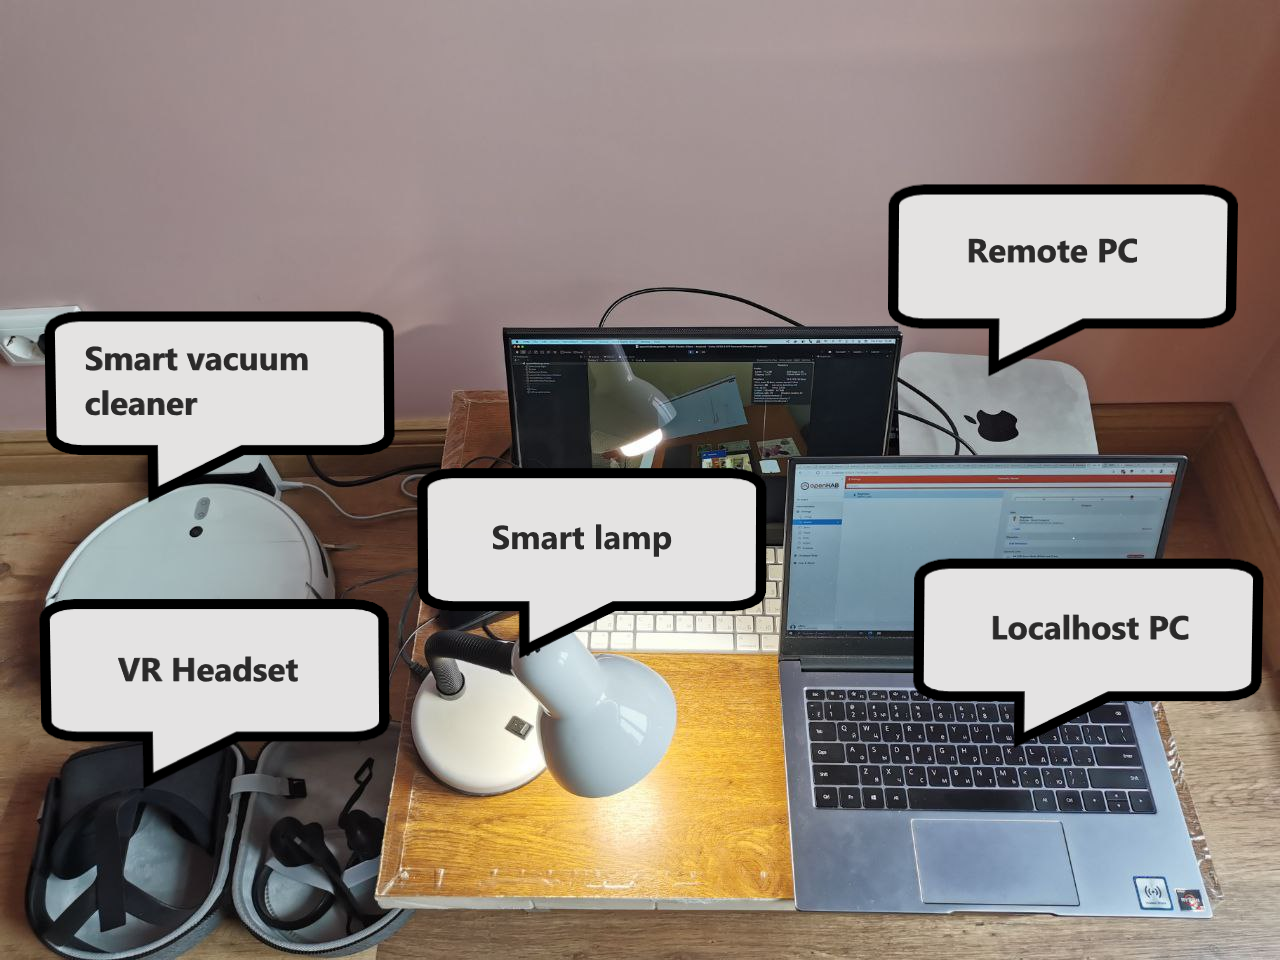
\includegraphics[width=0.9\linewidth]{figures/TestingEquipment.png}
  \caption{Testing equipment.}
  \label{fig:TestingEquipment-figure}
\end{figure}

The example research is on adding gesture control functionality for the smart lamp\footnote{Smart vacuum cleaner and remote PC will be used in the next experiment}.

The virtual environment provides Widgets for Light and Gesture Recognition. In other words, a virtual lamp should be equivalent to the real-world one and gesture interface should be implemented.

\section{Server setup}
Firstly, a binding needs to be added to the openHAB server. Xiaomi Mi IO binding makes it possible to automatically add the Xiaomi Smart Wi-Fi Lamp to the server (Figure~\ref{fig:ServerSetupProcedure-figure}).

\begin{figure}
  \centering
  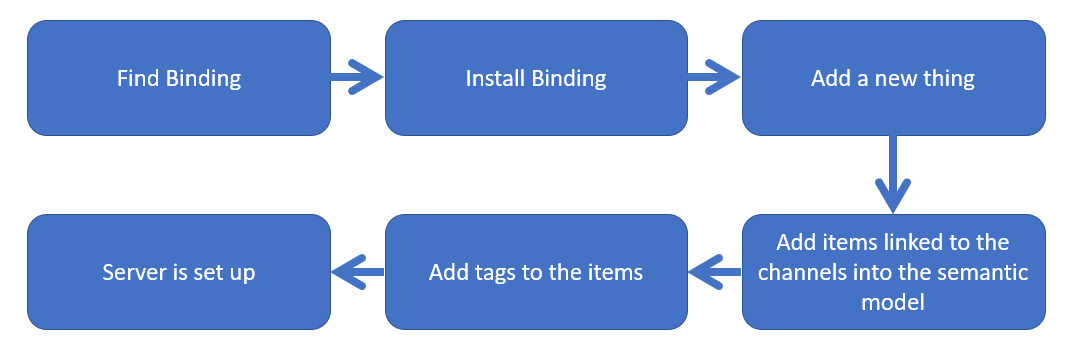
\includegraphics[width=0.9\linewidth]{figures/ServerSetupProcedure.png}
  \caption{Server setup procedure.}
  \label{fig:ServerSetupProcedure-figure}
\end{figure}

Next is adding items linked to the lamp channels. In the example the lamp brightness dimmer is added to the semantic model.

\begin{figure}
  \centering
  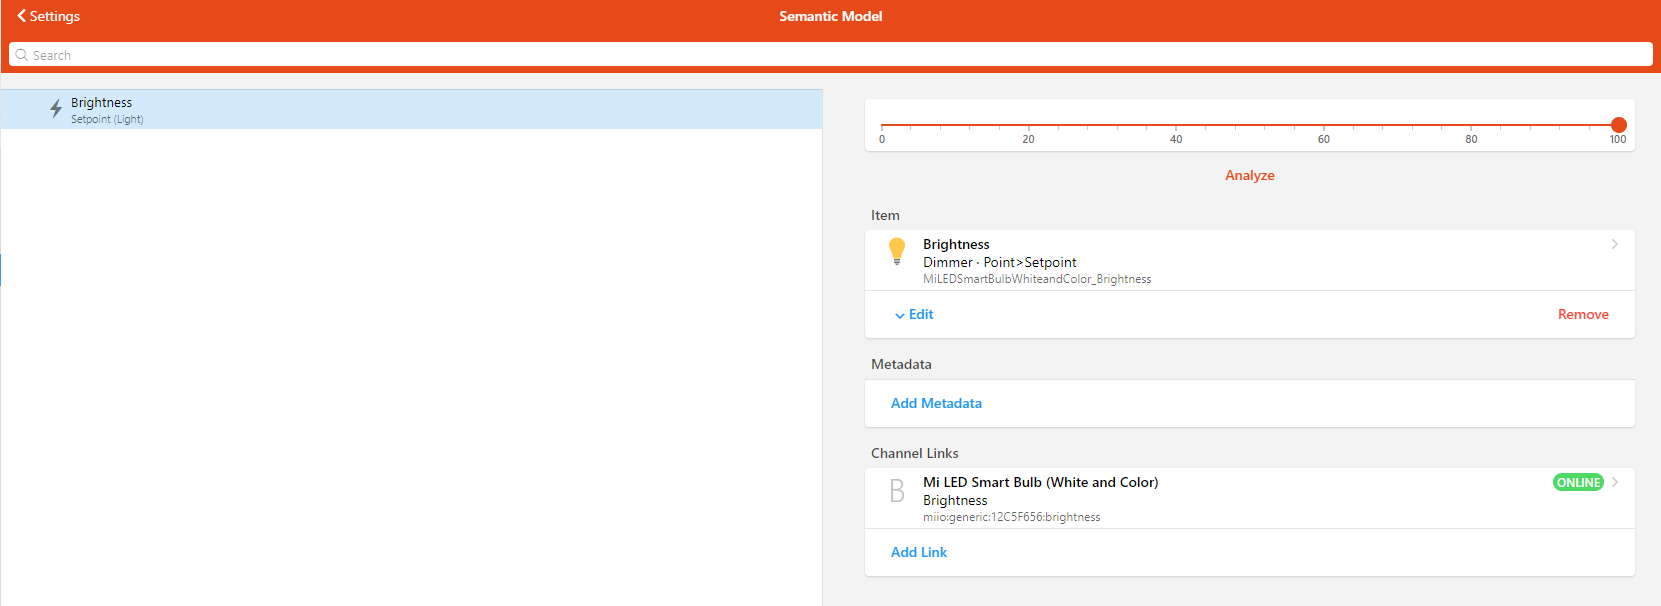
\includegraphics[width=0.9\linewidth]{figures/SemanticModelOne.png}
  \caption{Semantic model 1.}
  \label{fig:SemanticModelOne-figure}
\end{figure}

As seen on Figure~\ref{fig:SemanticModelOne-figure}, the brightness can be already controlled by moving the dimmer. The real-world lamp will change the brightness based on the value on the server.

Next step is adding tags to the item: the lamp should be controlled by Gestures, then a corresponding tag has to be added (Figure~\ref{fig:ItemEditPage-figure}).

\begin{figure}
  \centering
  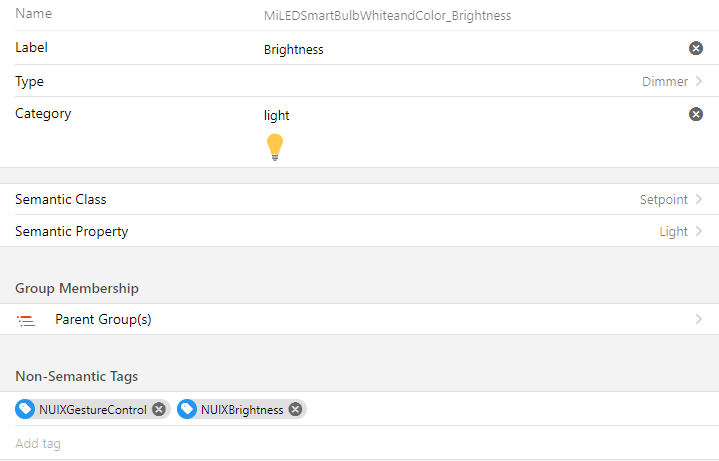
\includegraphics[width=0.9\linewidth]{figures/ItemEditPage.png}
  \caption{Item Edit Page.}
  \label{fig:ItemEditPage-figure}
\end{figure}

The server has been set up for connection to NUIX-Studio App instances.

\section{Running NUIX-Studio APP}

After the server has been set up, and the Smart home environment has been chosen, the platform is ready to run on the devices.

(A screenshot with gesture control).

In the experiment a VR-IoT platform user performs three tasks:
\begin{enumerate}
    \item Put on Virtual reality headset;
    \item Press the virtual button to establish a Client-Server connection and receive the items list;
    \item Perform a "Thumb up" gesture. By rotating the fist, the lamp brightness changes in the VR-IoT environment\footnote{Both in real and virtual worlds}.
\end{enumerate}

Данные действия были проделаны пользователем платформы. Таким образом, была добавлена поддержка жестов для управления яркостью лампы и эксперимент по созданию нового устройства для существующей среды можно считать успешным. 

\section{Performance analysis}

Анализ производительности платформы не является основной целью исследования, но тем не менее, он показателен с точки зрения нахождения бутылочных горлышек. Будет показано, что задачи рендеринга имеет смысл выполнять на отдельном сервере, а иметь общую базу данных для всех экземпляров приложения поможет добиться в итоге одновременной работы нескольких пользователей внутри системы.

The first experiment is the analysis of the system startup, performed on three devices by registering the startup time (Figure~\ref{fig:SystemStartupScheme-figure}).

\begin{figure}
  \centering
  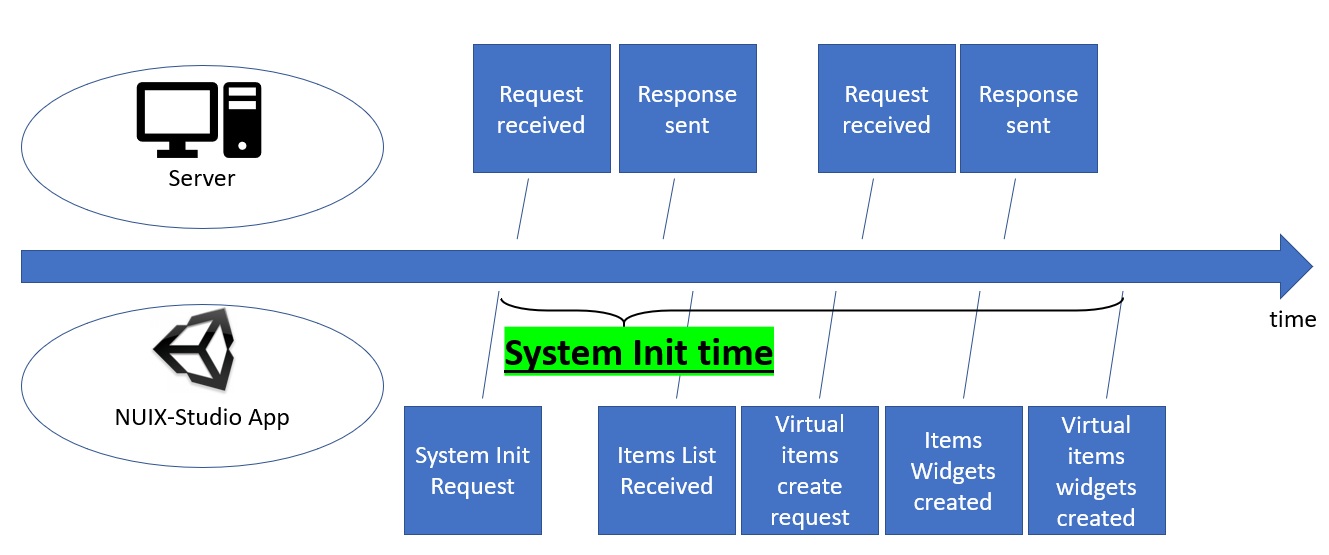
\includegraphics[width=0.9\linewidth]{figures/SystemStartupScheme.png}
  \caption{System startup scheme.}
  \label{fig:SystemStartupScheme-figure}
\end{figure}

The hardware specifications can be seen on Table~\ref{tab:hardware-specifications-table} \footnote{Localhost PC is a notebook running openHAB server as well as one instance of NUIX-Studio APP; Remote PC is a computer running one instance of NUIX-Studio APP and connected to the same Wi-Fi network as localhost PC; Oculus Quest is a Virtual Reality Headset running NUIX-Studio APP and connected to the same Wi-Fi network as PCs.}.

\begin{table}
  \centering
  \begin{threeparttable}[c]
    \caption{Hardware specifications in the experimental setup}
    \label{tab:hardware-specifications-table}
    \begin{tabular}{ll}
      \toprule
      Unit    &         Specifications                 \\
      \midrule
      Localhost PC & Ryzen 5 3500u, Windows 10 \\
      Remote PC & Core i5 4278U, macOS 11.2.3    \\
      Oculus Quest        & Qualcomm Snapdragon 835, Android-based            \\
      \bottomrule
    \end{tabular}
  \end{threeparttable}
\end{table}

Each test was performed on a new instance of Unity APP to avoid cashing influence. And then mean values have been calculated (Figure~\ref{fig:SystemInitTime-figure}).

\begin{figure}
  \centering
  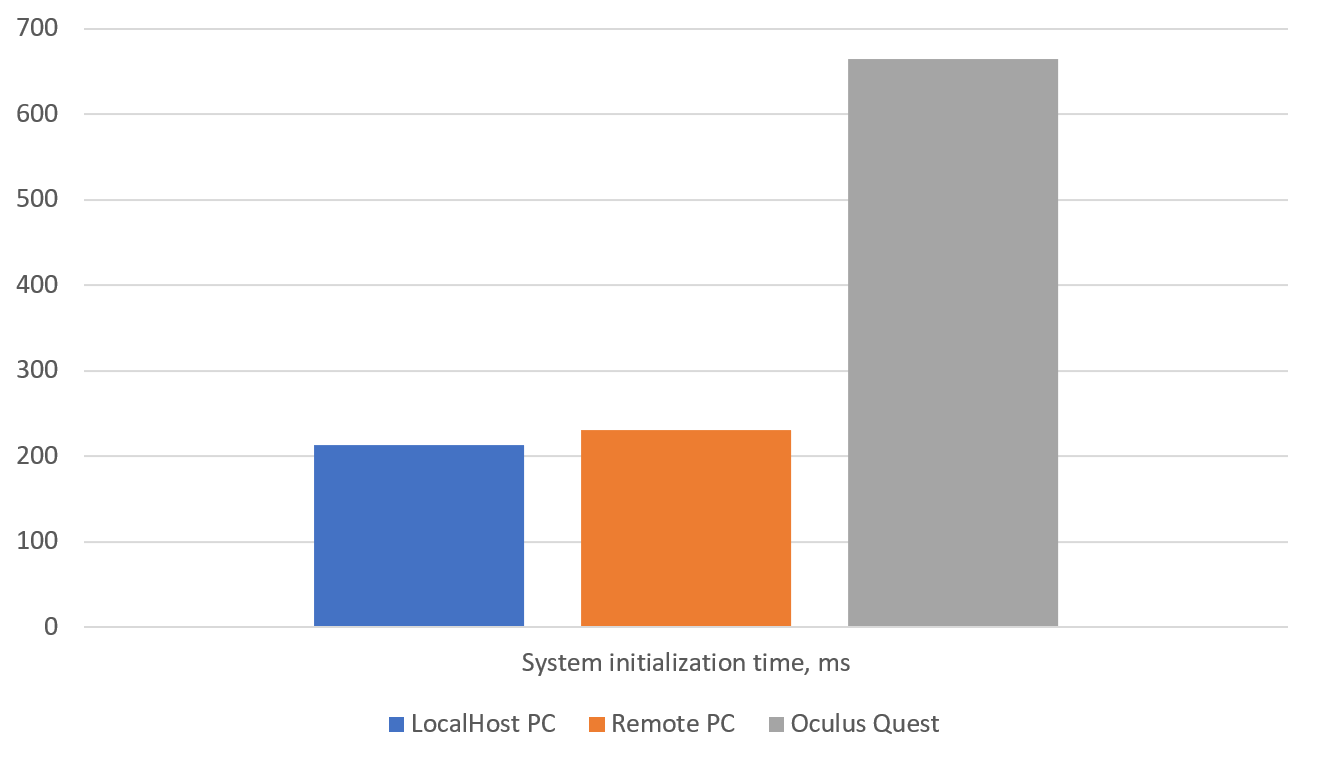
\includegraphics[width=0.9\linewidth]{figures/SystemInitTime.png}
  \caption{System initialization time measured on different client devices.}
  \label{fig:SystemInitTime-figure}
\end{figure}

As seen on Figure~\ref{fig:SystemInitTime-figure}, the system initialization time is a time-consuming operation, which from 200 to over 600ms in average to perform.

В следующем эксперименте производились замеры event processing time. На одном из устройств, на котором запущена NUIX-Studio App instance менялось значение Item\footnote{В данном случае меналась яркость умной лампочки by moving the corresponding pinch slider widget}. На сервере происходила обработка полученного запроса на изменения параметра Item, и на все устройства, подключенные к серверу, с запущенной NUIX-Studio App Instance, отправлялся Event, содержащий информацию о новом значении Item. Устройство, на котором произошло данное изменение Item, игнорировало новое поступившее значение, так как оно совпадает со старым значением. Объектом измерения же является время обработки запроса на другом устройстве (Figure~\ref{fig:EventProcessingScheme-figure}).

\begin{figure}
  \centering
  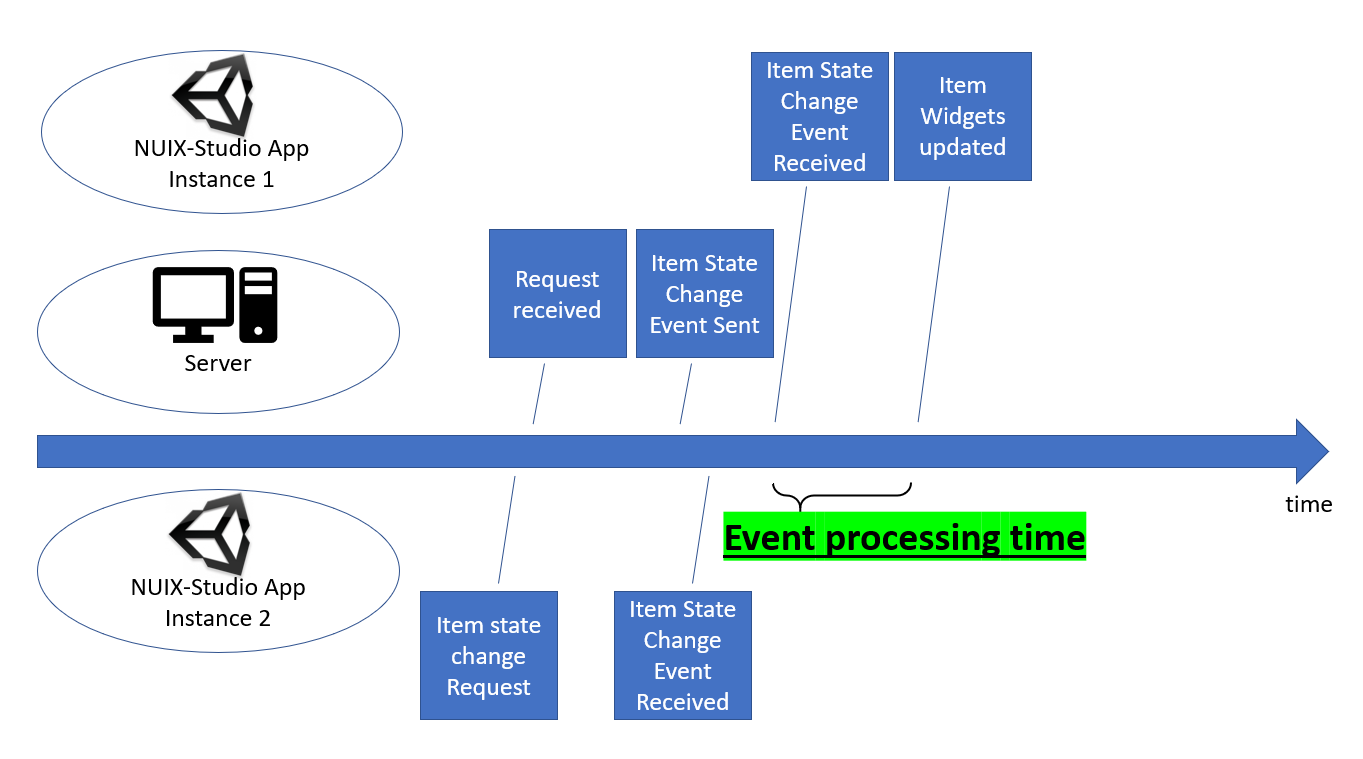
\includegraphics[width=0.9\linewidth]{figures/EventProcessingScheme.png}
  \caption{Event processing scheme.}
  \label{fig:EventProcessingScheme-figure}
\end{figure}

\begin{figure}
  \centering
  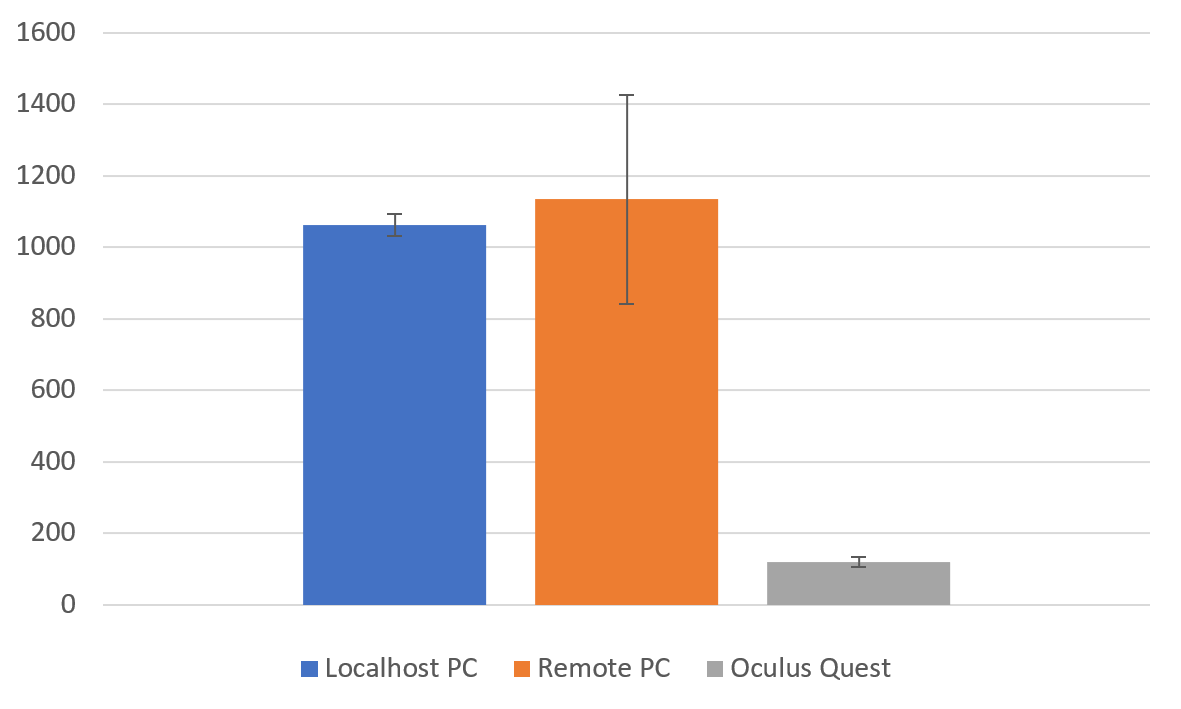
\includegraphics[width=0.9\linewidth]{figures/EventProcessingTime.png}
  \caption{Event processing time measured on different devices.}
  \label{fig:EventProcessingTime-figure}
\end{figure}

Как видно из полученной гистограммы (Figure~\ref{fig:EventProcessingTime-figure}), Oculus Quest performance on this test is outstanding: the event processing time is around 10 times lower compared to the PCs, which stands in confrontation with the assumption that this test is only device performance-based. One of the possible reasons of such results is optimization: NUIX-Studio APP is built for Oculus Quest, while on PCs it is run in the “Editor” mode, not built specifically for the platform.


Результаты данного эксперимента будут использованы в дальнейшем: System initialization time is time consuming and is based on the device hardware performance, and in some later experiments it is better to not perform time calculations that include system initialization, while event processing time is relatively low, and in most cases it can be neglected.

В следующем эксперименте используются шлем виртуальной реальности, умная лампочка и сервер с запущенным на нем приложением. Предположим, что внутри системы умного дома используется датчик света, который находится на относительно большом расстоянии от лампы (2-3 метра), и срабатывает, когда количество света, падающего на его датчик, превосходит некоторое пороговое значение. К примеру, такой setup иногда используется на предприятиях при первоначальной настройке освещения для нахождения грани между комфортным уровнем освещения и оптимальным уровнем энергопотребления. Датчик света будет срабатывать именно при некотором достаточно большом значении яркости лампы. Таким образом, нужна максимально точная настройка уровня яркости лампочки.

В предыдущем эксперименте было показано, что управление жестами возможно для контроля уровня яркости лампы. Покажем, что в данном случае перенос вычислений со шлема вирутальной реальности на сервер необходим. Задание пользователя состоит из тех же шагов, что и в предыдущем эксперименте, но при этом добавляется еще один шаг: точная настройка уровня яркости. Предположим, что датчик освещения срабатывает при уровне яркости лампочки 50 из 100\footnote{Данное число выбрано автором исследования случайно, без опоры на принципы fits law}. Задача пользователя как можно быстрее привести яркость лампочки в данное положение при помощи жестового управления. Для того, чтобы исключить дополнительные операции, не относящие к непосредственному использованию жестов для изменения яркости лампы, такие как запуск системы, подопытному было необходимо повторить шаг с приведением яркости лампы в заданное положение два раза. Время, между первым и вторым рахом, когда яркость лампы равнялась заданному значению, можно разделить на две составляющих (Equation \eqref{eq:totaltime}) : время реакции подопытного на успешное изменение уровня яркости $t_{foc}$, и время выполнения новой калибровки $t_{cal}$.

\begin{equation}
  t = t_{foc} + t_{cal}
  \label{eq:totaltime}
\end{equation}

В эксперименте участововало пять человек. Были произведены две серии опытов: в первой серии подсчет освещения лампы происходил на устройстве виртуальной реальности, а во второй - на сервере. На устройство виртуальной реальности же передавалась лишь информация, а именно карта света. В каждой серии опытов было произведено по двадцать пять замеров, и полученные данные были помещены на график (). Если учесть, что время фокусировки подопытного $t_{foc}$ - независимая от измененных параметров синхронизации величина, то разница между подсчитанным временем в первой и во второй серии опытов как раз будет равна разнице между временем, затраченным на калибровку яркости лампы в первой и во второй серии опытов. (Equation \eqref{eq:totaltime})

\begin{equation}
  t_{\delta} = (t_{foc} + t_{cal_1}) - (t_{foc} + t_{cal_1}) = t_{cal_1} - t_{cal_2}
  \label{eq:deltatime}
\end{equation}

Как видно из получившейся гистограммы, разница при выполнении функции калибровки в первом и во втором задании составляет 500 миллисекунд. Учитывая, что время обработки запроса, поступающего с сервера составляет не более 1 миллисекунды\footnote{Было получено в предыдущей главе}, видна колоссальная разница во времени выполнения.

Во время выполнения опыта также брались анализировались дополнительные данные, такие как количество кадров в секунду, с которыми происходила отрисовка изображения на экране. На графике () видно, что в первой серии опытов количество кадров в секунды значительно падает, как только происходит инициализация системы и создания виджетов для items from semantic model: с 72 кадров в секунду, что явяляется hardware ограничением шлема вирутальной реальности до 20 кадров в секунду. Во второй серии опытов такого падения уже не наблюдается (ссылка на график): благодаря тому, что подсчет освещения происходит на отдельном устройстве, количество кадров в секунду падает лишь незначительно с 72 до 65. Учитывая, что обработка hands recognition происходит не чаще 1 раза за кадр, то можно сделать предположение, что разница во времени как раз обусловлена задержкой в считывании жеста. Можно провести аналогию с мышкой: пользователь будет чаще попадать в нужную кнопку, если управление мышкой более отзывчивое. Тем не менее, основная хадача эксперимента заключалась в том, чтобы показать, как перенос ресурсоемких вычислений со шлема виртуальной реальности на сервер улучшает пользовательский опыт, одно из требований к построению VR-IoT Research platform. Таким образом, эксперимент можно считать успешным.


В следующем эксперименте была проверена гипотеза, возможна ли совместная работа в одной VR-IoT environment, посредством добавления новых IoT устройств в систему и изменения их параметров. Автор не останавливается подробно на обсуждении этой гипотезы, так как ее реузльтаты уже предугадывались из предыдущих экспериментов:
\begin{enumerate}
    \item Время добавления устройства в систему ограничено производительностью конкретной платформы, а также скоростью интернет соединения внутри Wi-Fi сети. При запуске 300 последовательных тестах ping от remote PC до localhost PC все полученные значения были меньше 100мс, при 90 процентах значений в диапазоне от 45мс до 70мс. Время же, затраченное устройством на создание виджетов для умного пылесоса примерно соотвествовало времени инициализации системы;
    \item Время от изменения Item на remote PC NUIX-Studio App Intance до получения remote PC подтверждения об соответствующих виджетов на localhost PC NUIX-Studio App Instance не превышало 60мс, при 90 процентах значений от 53мс до 80мс.
\end{enumerate}

Таким образом, скорость работы сети играет существенную роль в работе системы. Лишь при минимальных задержках сети, доступных уже сейчас в сетях Wi-Fi 6, а также в сетях 6G в будущем, будет затруднена simultaneous work inside the same VR-IoT environment. Тем не менее, было замечено, что такие операции, как добавление новых устройств в систему требуют ощутимых времязатрат. В связи с тем, что происходит запрос на создание игровых объектов, автор предполагает, что основная задержка связана именно с внутренними процессами внутри Unity 3D engine.

В следующей главе будет показано, как теоретически можно обойти данные ограничения.